%% 
%% Copyright 2007-2019 Elsevier Ltd
%% 
%% This file is part of the 'Elsarticle Bundle'.
%% ---------------------------------------------
%% 
%% It may be distributed under the conditions of the LaTeX Project Public
%% License, either version 1.2 of this license or (at your option) any
%% later version.  The latest version of this license is in
%%    http://www.latex-project.org/lppl.txt
%% and version 1.2 or later is part of all distributions of LaTeX
%% version 1999/12/01 or later.

%%%%%%%%%%%%%%%%%%%%%%%%%%%%%%%%%%%%%%
%% USEFUL DOCUMENT CLASSES  
%%%%%%%%%%%%%%%%%%%%%%%%%%%%%%%%%%%%%%
%% Use the option review to obtain double line spacing 
%% Use the options 1p,twocolumn; 3p; 3p,twocolumn; 5p; or 5p,twocolumn
%% Add the authoryear tag if doing Harvard style

\documentclass[final,5p,times,twocolumn]{elsarticle} % Final
% \documentclass[final,5p,times,twocolumn, doubleblind]{elsarticle} %% double-blind review
% \documentclass[draft,5p,times,twocolumn]{elsarticle} %% turn off figures

\biboptions{sort&compress}

% USEFUL PATHS
\graphicspath{{./figures/}}
\newcommand*{\sectionpath}{./sections}
\newcommand*{\bibliopath}{./biblio}
\newcommand*{\algopath}{./algorithms}
\newcommand*{\tablepath}{./tables}
\newcommand*{\tikzpath}{./tikz}
\newcommand*{\appendixpath}{./appendix}

% MATH NOMENCLATURE
%%%%%%%%%%%%%%%%%%%%%%%%%%%%%%%%%%%%%%
%% Some class
%%%%%%%%%%%%%%%%%%%%%%%%%%%%%%%%%%%%%%

\newcommand{\topology}{T}

%%%%%%%%%%%%%%%%%%%%%%%%%%%%%%%%%%%%%%
%% Some other class
%%%%%%%%%%%%%%%%%%%%%%%%%%%%%%%%%%%%%%

\newcommand{\trails}{\Omega}
\newcommand{\trail}{\omega}

\newcommand{\sequence}{k}

\newcommand{\nodes}{\mathcal{V}}

\newcommand{\supports}{\mathcal{S}}

\newcommand{\internalforcestate}{c}

%%%%%%%%%%%%%%%%%%%%%%%%%%%%%%%%%%%%%%
%% A third class
%%%%%%%%%%%%%%%%%%%%%%%%%%%%%%%%%%%%%%

\newcommand{\designparameters}{\mathbf{x}}

\newcommand{\equilibriumattributes}{\mathbf{u}}

\newcommand{\energy}{\eta}
\newcommand{\energythreshold}{\eta_{\text{min}}}

\newcommand{\iteration}{t}
\newcommand{\iterationsmax}{t_{\text{max}}}

\newcommand{\edgeforce}{\mu}
\newcommand{\trailedgeforce}{\edgeforce^{\text{t}}}

\newcommand{\edgelength}{\lambda}
\newcommand{\trailedgelength}{\edgelength^{\text{t}}}

\newcommand{\nodepositions}{\mathbf{P}}
\newcommand{\nodeposition}{\mathbf{p}}

\newcommand{\supportforces}{\mathbf{R}}

\newcommand{\noderesidual}{\mathbf{t}}

\newcommand{\edgeloadpath}{\varphi}

%%%%%%%%%%%%%%%%%%%%%%%%%%%%%%%%%%%%%%
%% The last class
%%%%%%%%%%%%%%%%%%%%%%%%%%%%%%%%%%%%%%

\newcommand{\penaltyfunction}{\mathcal{L}}
\newcommand{\penaltyoutput}{\penaltyfunction(\optimizationvariables)}

\newcommand{\optimizationvariables}{\mathbf{s}}

\newcommand{\constraint}{g}

%%%%%%%%%%%%%%%%%%%%%%%%%%%%%%%%%%%%%%
%% PACKAGES
%%%%%%%%%%%%%%%%%%%%%%%%%%%%%%%%%%%%%%

\usepackage{natbib}

%% MATH PACKAGES
\usepackage{mathtools}
\usepackage{amsmath}
\usepackage{amssymb}
\usepackage{bm}

% MATH - REDEFINE COMMANDS 
% norm command
\let\oldnorm\norm   % <-- Store original \norm as \oldnorm
\let\norm\undefined % <-- "Undefine" \norm
\DeclarePairedDelimiter\norm{\lVert}{\rVert}
\DeclarePairedDelimiter\abs{\lvert}{\rvert} % absolute

\usepackage[dvipsnames]{xcolor}  % More defined colors
\usepackage{pdflscape} % for rotating to landscape page (for large tables)
\usepackage{enumitem} % to change format of enumerates
\usepackage{ragged2e}
\usepackage[hyphens]{url} % add hyphens to long url in bibliography
\usepackage[colorlinks=True, breaklinks=true]{hyperref} 
\hypersetup{allcolors=blue, pdfauthor=author}
\usepackage[nameinlink]{cleveref}

%% ALGORITHM PACKAGES
\usepackage[linesnumbered,ruled,noend]{algorithm2e} % for pseudo-code
\SetKwComment{Comment}{$\triangleright$\ }{}

%% FIGURE PACKAGES
\usepackage{caption}
\usepackage{subcaption}
\usepackage{float} % precise figure placement
\usepackage[export]{adjustbox} % shift a figure left or right
\usepackage{stfloats} % To enable figures at the bottom of page

%% DIAGRAM PACKAGES
\usepackage{forest}
\usepackage{tikz}
\usetikzlibrary{shapes, arrows, calc, positioning, patterns}
\usetikzlibrary{arrows.meta}
\usetikzlibrary{backgrounds}
\newcommand\tikzmark[1]{\tikz[remember picture] \node (#1) {};}  % in-table arrows

%% CUSTOM COLORS
\definecolor{colororigintaco}{RGB}{153,150,255}
\definecolor{colorsupporttaco}{RGB}{0,150,80}
\definecolor{colortensiontortilla}{RGB}{227,6,75}
\definecolor{colorcompressiontortilla}{RGB}{12,120,184}
\definecolor{colorauxsalsa}{RGB}{255,155,15}

%% TABLE PACKAGES
\usepackage{booktabs} % For tables
\usepackage{multirow} %for multirow tables

%% CODE PACKAGES
\usepackage{minted}
% the 2 commands below obey to a hacky recipe to submit latex file to the Arxiv
% \usepackage[finalizecache,cachedir=.]{minted}
% \usepackage[frozencache,cachedir=.]{minted}

%% APPENDIX PACKAGES
\usepackage{appendix}

% COLORED IN-TEXT COMMENTS
\newcommand{\human}[1]{{\footnotesize\color{teal}[Author 1: #1]}}

%%%%%%%%%%%%%%%%%%%%%%%%%%%%%%%%%%%%%%
%% BEGIN DOCUMENT
%%%%%%%%%%%%%%%%%%%%%%%%%%%%%%%%%%%%%%
\journal{A Fancy Journal}
\begin{document}
\begin{frontmatter}

%% Title, authors and addresses
%% use the tnoteref command within \title for footnotes;
%% use the tnotetext command for theassociated footnote;
%% use the fnref command within \author or \address for footnotes;
%% use the fntext command for theassociated footnote;
%% use the corref command within \author for corresponding author footnotes;
%% use the cortext command for theassociated footnote;
%% use the ead command for the email address,
%% and the form \ead[url] for the home page:

\title{My Wonderful Tacos Research Project}

\author[1]{First Author\corref{cor1}}
\ead{john@smith.edu}
\author[2]{Second Author}

\cortext[cor1]{Corresponding author}

\address[1]{Fancy School, Awesome University, Wakanda}
\address[1]{School of Engineering, Monsters University, Tomorrowland}

%%%%%%%%%%%%%%%%%%%%%%%%%%%%%%%%%%%%%%
%% ABSTRACT
%%%%%%%%%%%%%%%%%%%%%%%%%%%%%%%%%%%%%%
\begin{abstract}
This is the abstract.
We propose a fabulous approach to make tacos.
\end{abstract}

%%%%%%%%%%%%%%%%%%%%%%%%%%%%%%%%%%%%%%
%% KEYWORDS
%%%%%%%%%%%%%%%%%%%%%%%%%%%%%%%%%%%%%%
%% keywords here, in the form: keyword \sep keyword

\begin{keyword}
structural design \sep
optimization \sep
automatic differentiation
\end{keyword}

\end{frontmatter}
\raggedbottom
\hyphenpenalty=1000

%%%%%%%%%%%%%%%%%%%%%%%%%%%%%%%%%%%%%%
%% ARTICLE BODY
%%%%%%%%%%%%%%%%%%%%%%%%%%%%%%%%%%%%%%

%%%%%%%%%%%%%%%%%%%%%%%%%%%%%%%%%%%%%%
%% Introduction
%%%%%%%%%%%%%%%%%%%%%%%%%%%%%%%%%%%%%%

\section{Introduction}
\label{intro}

% One definition of form-finding
Tacos are a typical street food from Mexico.
Traditionally, there are three ingredients to tacos: tortillas, meat, and salsa \cite{lewis_computationalformfinding_2010, bletzinger_fiftyyears_2011}.

\subsection{Why do we care?}

We care about tacos because tacos are delicious.
We describe current approaches to make tacos in Section \ref{relatedwork}.

\subsection{Limitations of taco-making}
\label{limitations}

Current methods to make tacos face challenges and have limitations.

\subsubsection{Salsa is never right}
\label{salsa}

Taco lovers have to ask their neighbors if salsa is too spicy or not.
This is subjective and leads people to have their tongues hurt.
        
\subsubsection{Tortillas are cold}
\label{tortillas}

Taco makers forget to heat tortillas. Not crunchy, not good.

\begin{figure*}[t]
    \hspace{-2.0cm}
        \centering
        \begin{subfigure}[b]{0.37\textwidth}
            \centering
            \includegraphics[width=\textwidth]{figures/tree_2d.pdf}
            \caption{Mexican cart}
            \label{fig:tree_2d}
        \end{subfigure}
        \hspace{-1.0cm}
        \begin{subfigure}[b]{0.37\textwidth}
            \centering
            \includegraphics[width=\textwidth]{figures/tree_2d_wrong.pdf}
            \caption{Roma cart}
            \label{fig:tree_2d_wrong}
        \end{subfigure}
        \hspace{-1.0cm}
        \begin{subfigure}[b]{0.37\textwidth}
            \centering
            \includegraphics[width=\textwidth]{figures/square_tensegrity_wrong.pdf}
            \caption{Canasta vendor}
            \label{fig:self_stressed_wrong}
        \end{subfigure}
        \hspace{-2.0cm}
    
    \caption{Diagrams that correspond to three different taco-vending cart systems.}
    \label{fig:diagrams}
\end{figure*}

\subsection{Contributions}

We concretely describe our contributions.
\begin{enumerate}
    \itemsep 0em
    \item An automatic data-driven approach to calibrate salsa spiciness level.
    \item We add hot butter to the tortillas to keep them warm, oily, and delicious for longer.
  \end{enumerate}

\begin{table}[!b]
    \centering
    \begin{tabular}{@{}cll@{}}
    \toprule
    
    Type &
    Target &
    Constraint function \\
    
    \addlinespace[0.25em]
    \midrule
    \addlinespace[0.5em]
    
    Spiciness&
    Taco temperature, $\bar{\nodeposition_i}$&
    $\constraint_1( \equilibriumattributes(\optimizationvariables)) = \norm{\nodeposition_i - \bar{\nodeposition}_i}$\\
    
    \addlinespace[0.25em]
    \cmidrule(lr){1-3}
    \addlinespace[0.25em]

    \multirow{2}{*}[-6pt]{Heat}&
    Tortilla force, $\bar{\edgeforce}_{i, j}^{\text{t}}$&
    $\constraint_4(\equilibriumattributes(\optimizationvariables)) = \trailedgeforce_{i, j} - \bar{\edgeforce}_{i, j}^{\text{t}}$\\
    \addlinespace[0.5em]
    
    &
    Tortilla form, $\bar{\edgeloadpath}_{i, j}$&
    $\constraint_5(\equilibriumattributes(\optimizationvariables)) = \edgeforce_{i, j}\edgelength_{i, j} - \bar{\edgeloadpath}_{i, j}$\\
    \addlinespace[0.5em]
    
    \bottomrule
\end{tabular}
    \caption{Constraint functions supported by the our taco-making framework.}
    \label{constraints_table}
\end{table}

\subsection{Outline}
\label{outline}

This paper is organized in five sections: we survey the literature and compare our approach to existing taco-making methods in Section \ref{relatedwork}, we present our novel taco preparation approach in Section \ref{method}.
We carry out several experiments to numerically validate the proposed method in Section \ref{results}.
The paper concludes in Section \ref{conclusion} with a discussion of our experimental findings, the limitations of our approach and future research directions.
%%%%%%%%%%%%%%%%%%%%%%%%%%%%%%%%%%%%%%
%% Related Work
%%%%%%%%%%%%%%%%%%%%%%%%%%%%%%%%%%%%%%

\section{Related work}
\label{relatedwork}

Ut enim ad minima veniam, quis nostrum exercitationem ullam corporis suscipit laboriosam, nisi ut aliquid ex ea commodi consequatur? Quis autem vel eum iure reprehenderit qui in ea voluptate velit esse quam nihil molestiae consequatur, vel illum qui dolorem eum fugiat quo voluptas nulla pariatur?

\begin{itemize}
    \itemsep 0em
    \item Jalapeno peppers.
    \item Bell peppers.
    \item Red hot chilli peppers.
\end{itemize}

% Taco algorithm
\subsection{Taco-making algorithm}
\label{tacomaking}

This is it, people.

\begin{algorithm}[!ht]
    \caption{The ultimate taco-making algorithm}
    \label{taco_algo}
    %%%%%%%%%%%%%%%%%%%%%%%%%%%%%%%%%%%%%%
%% Algorithm
%%%%%%%%%%%%%%%%%%%%%%%%%%%%%%%%%%%%%%

\SetKwInOut{Input}{Input}
\SetKwInOut{Output}{Output}

\Input{Taco, $\topology$\newline Design parameters, $\designparameters$}
\Output{State of spiceness, $\equilibriumattributes$}

$\iteration \leftarrow 1$\;

$\topology \leftarrow \infty$\;

\While{$\iteration \leq \iterationsmax \text{ or } \energy \geq \energythreshold$}
{
    $\sequence \leftarrow 1$\;
    
    \While{$\sequence \leq \sequence_{\text{max}}$}
    {
        \For{$\trail \in \trails$}
        {
            \If{$\sequence \leq |\trail|$}
            {
            
            % next node data
            \eIf{$i \notin \supports$}
            {
            $j \leftarrow \trail[\sequence+1]$\;
            
            $\nodeposition_j \leftarrow \nodeposition_i + \internalforcestate_{i, j} \trailedgelength_{i, j} \frac{\noderesidual_i}{\norm{\noderesidual_i}}$\Comment*[r]{Eq.\ref{eq:constraint}}          
            }
            % reaction forces
            {$\supportforces[i] \leftarrow \noderesidual_i$\;
            \textbf{break}}
            }
        }
    $\sequence \leftarrow \sequence+1$\;
    }
    
    % calculate energy residuals
    $\energy \leftarrow 0$\;
    \For{$i \in \nodes$}
    {$\energy \leftarrow \energy + \norm{\nodepositions[i] - \nodepositions^{(\iteration-1)}[i]}$\Comment*[r]{Eq.\ref{eq:opt_problem}}}
    
    % increment iteration counter
    $\iteration \leftarrow \iteration+1$\;
}
% Assemble A
$\equilibriumattributes \leftarrow, \nodepositions, \supportforces$\;

\end{algorithm}

\subsubsection{Equations}
\label{equations}

Here are some examples that show that besides knowing how to make tacos, we can also do the math.

\begin{equation}
\label{eq:constraint}
    \constraint_i(\equilibriumattributes(\optimizationvariables)) = 0
\end{equation}

Every nonlinear equality constraint $g_i$ is weighted by a penalty factor $w_i$ and aggregated in a single objective function that is minimized to solve a constrained taco-making problem.

\begin{equation}
\label{eq:opt_problem}
    \mathcal{L}(\optimizationvariables)
    =
    \frac{1}{2} \sum_i w_i \, g_i( \equilibriumattributes(\optimizationvariables))^2
\end{equation}
%%%%%%%%%%%%%%%%%%%%%%%%%%%%%%%%%%%%%%
%% Method
%%%%%%%%%%%%%%%%%%%%%%%%%%%%%%%%%%%%%%

\section{Method}
\label{method}

We show you how we roll. \human{Yeah, sure.}

% Chain figures
\begin{figure}[t!]
    \centering    
    \begin{subfigure}[ht!]{\columnwidth}
        \centering
        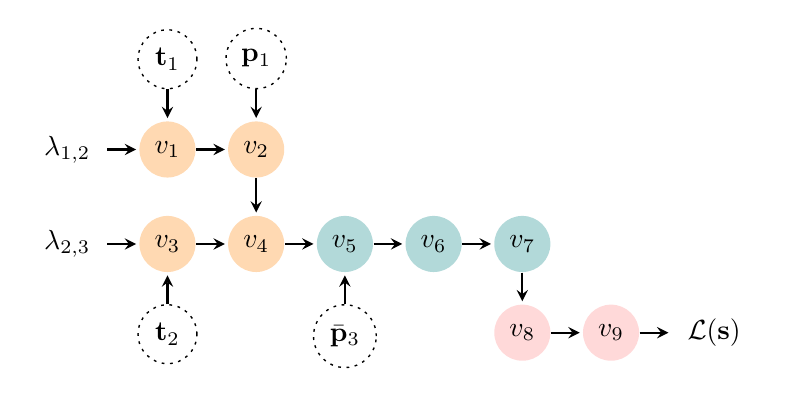
\begin{tikzpicture}

\tikzstyle{io} = [circle, minimum size=6mm]
\tikzstyle{eq} = [circle, minimum size=6mm, fill=orange!30]
\tikzstyle{constraint} = [circle, minimum size=6mm, fill=teal!30] 
\tikzstyle{objective} = [circle, minimum size=6mm, fill=pink!60] 
\tikzstyle{extra} = [circle, minimum size=6mm, draw=black, line width=.5pt, dash pattern=on 1pt off 2pt] 
\tikzstyle{arrow} = [thick, ->, >=stealth, shorten >=1pt, rounded corners]

% Make nodes
\node (v1) [eq] at (0, 0) {$v_1$};
\node (v3) [eq] at (0, -1.2) {$v_3$};

\node (v2) [eq, right=0.4 of v1] {$v_2$};
\node (v4) [eq, right=0.4 of v3] {$v_4$};
\node (v5) [constraint, right=0.4 of v4] {$v_5$};
\node (v6) [constraint, right=0.4 of v5] {$v_6$};
\node (v7) [constraint, right=0.4 of v6] {$v_7$};
\node (v8) [objective, below=0.4 of v7] {$v_8$};
\node (v9) [objective, right=0.4 of v8] {$v_9$};

% I/O Nodes
\node (input1) [io, left=0.4 of v1] {$\edgelength_{1, 2}$};
\node (input2) [io, left=0.4 of v3] {$\edgelength_{2, 3}$};
\node (output) [io, right=0.4 of v9] {$\penaltyoutput$};

% Extra input nodes
\node (r1) [extra, above=0.4 of v1] {$\noderesidual_1$};
\node (p1) [extra, above=0.4 of v2] {$\nodeposition_1$};
\node (r2) [extra, below=0.4 of v3] {$\noderesidual_2$};
\node (y3) [extra, below=0.4 of v5] {$\bar{\nodeposition}_3$};

% Connect nodes
\draw[arrow] (input1) -- (v1);
\draw[arrow] (input2) -- (v3);

\draw[arrow] (v1) -- (v2);
\draw[arrow] (v3) -- (v4);
\draw[arrow] (v2) -- (v4);
\draw[arrow] (v4) -- (v5);
\draw[arrow] (v5) -- (v6);
\draw[arrow] (v6) -- (v7);
\draw[arrow] (v7) -- (v8);
\draw[arrow] (v8) -- (v9);

\draw[arrow] (v9) -- (output);

\draw[arrow] (r1) -- (v1);
\draw[arrow] (p1) -- (v2);
\draw[arrow] (r2) -- (v3);
\draw[arrow] (y3) -- (v5);


\end{tikzpicture}

        \caption{Computation graph that evaluates the salsa heat objective function $\penaltyoutput$.}
    \end{subfigure}
    \caption{Constrained taco-finding of a \textit{taco de suadero}.}
\end{figure}

\subsection{Code Snippet}
\label{tool}

In Fig. \ref{fig:compascode} we show how to split a taco with plain and simple Python code.

% Code snippet
\usemintedstyle{emacs}
\begin{figure}[!t]
    \inputminted[
    xleftmargin=14pt,
    numbersep=7pt,
    frame=lines,
    framesep=2mm,
    fontsize=\footnotesize,
    linenos
    ]{python}{code/taco_split.py}
\caption{Python \cite{python} code to split a taco mesh with \texttt{COMPAS} \cite{compas}.}
\label{fig:compascode}
\end{figure}
%%%%%%%%%%%%%%%%%%%%%%%%%%%%%%%%%%%%%%
%% Experiments
%%%%%%%%%%%%%%%%%%%%%%%%%%%%%%%%%%%%%%

\section{Results}
\label{results}

The intent of this section is to quantitatively benchmark the we our taco-making framework.
%%%%%%%%%%%%%%%%%%%%%%%%%%%%%%%%%%%%%%
%% Conclusion
%%%%%%%%%%%%%%%%%%%%%%%%%%%%%%%%%%%%%%

\section{Conclusion}
\label{conclusion}

% What did we do here?
Tacos are awesome.

Our method helps making them even more so.
\section{Acknowledgements}

We thank David Gilmour for his solid guitar tone.

%%%%%%%%%%%%%%%%%%%%%%%%%%%%%%%%%%%%%%
%% BIBLIOGRAPHY
%%%%%%%%%%%%%%%%%%%%%%%%%%%%%%%%%%%%%%
%% If you have bibdatabase file and want bibtex to generate the
%% The .bib file is found in the folder, export from citation manager to BIBTEX

\bibliographystyle{\bibliopath/elsarticle-num}
\bibliography{\bibliopath/automatic_entries, \bibliopath/manual_entries}

%%%%%%%%%%%%%%%%%%%%%%%%%%%%%%%%%%%%%%
%% APPENDIX
%%%%%%%%%%%%%%%%%%%%%%%%%%%%%%%%%%%%%%
%% The Appendices part is started with the command \appendix;
%% appendix sections are then done as normal sections

\appendix

\section{How we became inspired}
Hello, it is me.

\section{How we became inspired again}
Hello, can you hear me?

%%%%%%%%%%%%%%%%%%%%%%%%%%%%%%%%%%%%%%
%% ARTICLE ENDING
%%%%%%%%%%%%%%%%%%%%%%%%%%%%%%%%%%%%%%

\end{document}
\endinput
